\chapter{Executing Relay}
\label{ch:execute}

Once a Relay program has gone through all optimization
  and lowering passes we must execute it.
In theory a naive interpretation strategy could be applied
    to the entire Relay program.
In fact the Relay definitional interpreter
  implements a naive recursive AST traversal
  which applies JIT compilation to each kernel invocation
  contained in the program.
A definitional interpreter is sufficient
  for specifying the behavior of a language,
  but not necessarily for efficiently executing one.
After applying generic optimizations,
  most compilers have per target compilation
  pipelines which lower programs to a specific
  backend.
Many of the behaviors contained in these target
  specific lowered programs require not only
  program transformations but also runtime
  support such as memory allocation,
  device selection, or scheduling.
The remainder of this chapter focuses on the backend
  of the Relay compiler and its runtime mechanisms.
We describe the general backend compilation strategy,
  lowering Relay to the graph runtime, the virtual machine,
  ahead of time compiler, and hardware accelerators.
In this chapter we evaluate Relay's performance specifically
  on state-of-the-art NLP applications and demonstrate
  state-of-the-art performance out performing leading industry standards
  such as TensorFlow and PyTorch.

\section{Compiler Framework}

To begin we first refresh the reader on the end-to-end
  dataflow of the Relay compiler.
First, a frontend converts its input format into the Relay IR.
Next, the Relay compiler typechecks and optimizes the program.
Processes such as automatic differentiation can be performed
  during this step.
Next we extract primitive functions
  from the Relay program, functions which may be lowering to TE or TIR,
  the process for selecting these
  is defined in Section \ref{sec:fusion}.
We then schedule and lower these
  expressions to produce low-level target-specific versions
  of these functions.
We then further transform the code which cannot be lowered
  into TIR via a sequence of passes depending on which backend
  we are targeting.
Finally we execute the remaining Relay code via a TVM runtime
  either the interpreter, which directly interprets the AST,
  the virtual machine, graph runtime, or native compiler all
  of which requires separate compilation phases.
The focus of this chapter is describing this process in
  detail for each compilation and runtime target.

\subsection{Frontend}

There are several ways to write an Relay program.
A user can build an in-memory representation of
    a program in C++, Rust or Python,
    parse one written in the Relay text format,
    load one from the on-disk serialization format,
    or import one from popular frameworks and interchange formats
    (e.g., TensorFlow, MxNet, Keras, DarkNet, and ONNX).
Many frameworks and interchange formats use static computation graph-based representations,
    which can easily be translated into Relay.
A greater challenge is translating frameworks
    with a richer computation model such as TensorFlow (TF).
TF supports control flow and includes \verb|TensorArray|, a write-once
    tensor container.
We can extract the loop structure out of a TensorFlow graph, converting
    it to an Relay loop, and transform the \verb|TensorArray| into an Relay list.
Many "importers" struggle to translate TensorFlow's full graph as their intermediate representation
  is not rich enough to capture the full IR, and often result in ad-hoc hacks to replicate
  TensorFlow's behavior.
Once new deep learning languages and IRs under development
    are stable it is likely that they can all be translated into Relay (see
    Section~\ref{sec:pl_techniques_in_dl}).
PyTorch provides an expressive programming model, and is a good fit
    for Relay, which has been previously integrated into PyTorch's
    \footnote{\url{https://github.com/pytorch/tvm}}
    \footnote{PyTorch engineers built an integration which connects PyTorch's backend to TVM.}
    JIT infrastructure, enabling users to transparently use Relay for improved performance.

\subsection{Compiler}
Once an Relay abstract syntax tree (AST) is produced,
    the program is optimized by applying a series of Relay-to-Relay
    passes.
Between each pass, Relay performs type inference and checking,
    rejecting malformed programs as well as populating shape and type
    information that passes can utilize.
The Relay compiler supports traditional optimizations
    (e.g., constant folding, common subexpression elimination, and dead code elimination)
    and domain-specific optimizations, see Chapter~\ref{ch:related} for more details.

\subsection{Runtimes}

Relay produces machine-specific code
    by decomposing the problem of code generation into multiple distinct phases.
Relay translates all operators into \tvm expressions
    to produce dense linear algebra kernels~\citep{tvm_osdi18, tensor_comprehensions, halide}.
\tvm produces low-level operators that expect a fixed calling convention,
    as well as preallocated inputs and outputs.
The result is an object file containing hardware-specific implementations of all
    operations.
The remaining Relay program then is executed or compiled,
    with operator invocations replaced by calls to the optimized operators.
By representing operators as \tvm expressions, we can programmatically
    transform them and automatically generate new implementations for the transformed operators.
Optimizations like fusion and quantization
    rely on this novel behavior.
After primitive operators are lowered,
    the remaining Relay program ties
    together operator invocations, allocation, control-flow,
    recursion, and high-level data structures.
There are multiple options for executing the combined full program:
    the Relay interpreter (with JIT compilation),
    an Relay virtual machine,
    the \tvm graph runtime,
    and an experimental Relay ahead-of-time compiler
    that converts programs to C++ to produce a target-specific binary.

\section{Interpreter \& Graph Runtime}
\label{sec:interp_graph_rt}

In the tradition of definitional interpreters we introduced
  a simple interpreter for Relay which implements its formal semantics, which
  we have separately formalized.
Relay’s interpreter can execute the full language but has notable limitations
  that make it unsuited for production deployments.
It is structured as an inefficient interpreter that performs
  AST traversal to execute the program.
Each time we want to run a sub-expression we must traverse each child node
  a large cost that can be easily avoided.
This approach is conceptually simple but inefficient, as
  the AST traversal heavily relies on indirection.
Furthermore we perform JIT compilation with concrete observed shapes
  in the interpreter, a flexible, but also costly choice.
For example the initial Relay prototype reused the existing ``graph runtime'', to obtain
  acceptable performance for vision tasks.
The graph runtime is heavily over engineered for completely static
  models.
The graph runtime can only execute simple control-free,
    DAGs of operations.
We can optimize Relay programs and map a subset of them
    to the graph runtime, but any use of new Relay features
    are unsupported.
The graph runtime does not support control-flow, dynamic shapes,
  recursion, closures, or data structures.

\section{Virtual Machine}
\label{sec:vm}

Existing approaches to dynamic model optimization apply or extend existing
  deep learning frameworks~\citep{xu2018cavs, gao2018low, yu2018dynamic, jeong2018improving, jeong2019janus, dynet, tf_fold}.
As discussed in Section~\ref{sec:dl_frameworks} frameworks are large monolithic pieces
  of software with both portability and performance challenges.
Existing work which builds on frameworks extends the programming model either
  via sophisticated additions~\citep{yu2018dynamic} or significant
  runtime overhead~\citep{tf_fold, jeong2019janus}.
Other work~\citep{xu2018cavs, gao2018low, tf_fold} which is focused on
  optimizing specific types of models is hard to generalize to new models,
  or generalize over all models.
Moreover, approaches which inherit from frameworks rely on third-party kernel
  libraries such as OpenBLAS~\citep{xianyi2014openblas},
  cuDNN~\citep{cudnn}, and MKL-DNN~\citep{mkldnn} to achieve competitive performance.
These libraries expose a fixed set of operators for the corresponding hardware,
  compromising the portability of dynamic models which require a large number of i
  specialized operators with varying data types and shapes.
Designing a new interface independent of existing frameworks
  provides a clean programming model but often at the cost of performance,
  due to dynamic interpretation of the model~\citep{dynet}.
Due to our ability to design a new IR and extensions for dynamic features
  we solve the majority of these challenges via the use of compilation.
Even though we can elide dynamism in many cases, there are still
  programs which need truly dynamic features, especially in more
  advanced scenarios like training.
To this end, we designed Relay VM, a high-performance and
  portable system for executing compiled dynamic neural networks
  on multiple platforms.

\subsection{A Tensor Virtual Machine}

TVM although named Tensor Virtual Machine, follows in the lineage of LLVM
  where its name is technically inaccurate.
In fact this is the first abstract or virtual machine introduced to the
  TVM compiler stack.
The Relay VM is a realization a tensor abstract machine,
  where each operation corresponds to high-level tensor operations such
  as allocating a tensor, invoking an operation like conv2d, or performing a device copy.
Conventional deep learning runtimes, those which apply interpretation of the
  computation graph by walking each node in topological order, are non-optimal
  for dynamic neural networks.
These interpreters are reminiscent of the earliest
  languages interpreters where the input language is directly
  processed to execute the program.
Due to the introduction of Relay programs containing
  control flow, recursion, dynamic shapes, and dynamic allocation,
  we must change how execution works.
The interpreter offers simple solutions for these,
  but none is sufficiently compelling or optimized.
The simplicity of the graph runtime provides attractive
  properties such as simple serialization, straightforward
  optimal memory layout, and ease of deployment.
An alternative solution to the VM is ahead of time
  compilation, we discuss below.

Virtual machine (VM) design is a
  well-studied area in programming languages and systems,
  and there have been various virtual machine designs
  for both full-fledged and embedded programing languages.
VMs provide are a sweet spot between
  poorly optimized naive interpreters
  and full ahead of time compilers.
The key advantage of VMs is the flexibility provided
  by having fine grained control over program execution.
For example dynamic scheduling or customized observability
  is much easier in the virtual machine setting vs. ahead of time compilation.

The Relay VM's design differs from traditional language VMs.
Traditional language VM designs have been heavily
  tailored to the execution profile of traditional programs.
Traditional programs manipulate small scalar values
  and consist of a large number of low-level instructions.
The sheer quantity of instructions requires instruction execution
  and dispatch to be extremely efficient.
Any instructions that don't directly correspond to the high-level
  instruction, such as managing VM state, or dynamic type tests
  are overhead.
In the context of machine learning we manipulate primarily tensor values,
  using a (relatively) low number of high level instructions.
ML programs’ cost centers are expensive operator invocations,
  such as GEMM or convolution, over a large input.
In this setting invoking the wrong kernel, or invoking a kernel inefficiently
  is the essential overhead.
Due to the execution profile exhibited by ML programs,
  micro-optimizations present in scalar VMs are dramatically less important,
  and thus the removal of dispatch overhead from ahead of time compilation
  is also less important.

\subsection{VM Compiler}

% TODO PUT IN FIGURE

In order to execute on the VM we wrote a new compiler which
  can lower Relay directly on to the VM bytecode, and then
  executed.
The compiler performs a set of transformations on the high-level
  Relay program before generating code:
\begin{itemize}
  \item A-Normal Form, converts program in to a limited single-assignment form.
  \item Lambda Lift, converts inline functions into top-level definitions,
        ensuring that capture lists are now explicit.
  \item Inline Primitives, ensures that fused functions are inlined into
        the program to enables simplified code generation.
  \item Inliner, general function inlining.
  \item Constant Pool Layout, traverse program collecting all constant values
        and layout them out in memory.
  \item ADT Tag Allocation, allocate the tag assignment for compilation
        to the VM.
\end{itemize}

\subsection{VM ISA}

\begin{table*}[h!]
    \begin{tabular}{@{}p{0.15\textwidth}p{0.375\textwidth}p{0.1\textwidth}p{0.375\textwidth}@{}}
    \toprule
    Instruction    & Description                                                  \\\midrule
    Move           & Moves data from one register to another.                     \\
    Ret            & the object in register result to caller's register.          \\
    Invoke         & Invokes a function at an index.                              \\
    InvokeClosure  & Invokes a Relay closure.                                     \\
    InvokePacked   & Invokes the function including operator kernel.              \\
    AllocStorage   & Allocates a storage block.                                   \\
    AllocTensor    & Allocates a tensor value of a certain shape.                 \\
    AllocTensorReg & Allocates a tensor based on a register.                      \\
    AllocADT.      & Allocates a data type using the entries from a register.     \\
    AllocClosure   & Allocates a closure.                                         \\
    GetTag         & Gets the tag of an Algebraic Data Types (\texttt{ADT}) cstr. \\
    GetField       & Gets the value at a certain index from an VM object.         \\
    ReshapeTensor  & Changes the shape of a tensor without altering its data.     \\
    If             & Jumps to the true or false offset with a condition.          \\
    Goto           & Unconditionally jumps to an offset.                          \\
    LoadConst      & Loads a constant at an index from the constant pool.         \\
    LoadConsti     & Loads a constant immediate.                                  \\
    DeviceCopy     & Copies a chunk of data from one device to another.           \\
    ShapeOf        & Retrieves the shape of a tensor.                             \\
    Fatal          & Raises fatal in the VM.                                      \\
    \bottomrule
    \end{tabular}
    \caption{The opcode and the description of the Relay instruction set \label{tab:isa}}
\end{table*}


After performing the above optimization pipeline the VM compiler
  itself is relatively straightforward.
The transformed program has a nearly one to one correspondence
  with the VM ISA.
The VM ISA is detailed in detail in the above figure.

The Relay dialect we transform the program into
  is designed to closely match the ISA, as discussed in Chapter~\ref{ch:optimizations}.
The VM's ISA is motivated by our previous observation that
  kernel execution dominates neural network execution time.
If we treat kernel invocation as a single instruction,
  the cost of surrounding instructions is negligible in the total execution.
As a result, our design is quite different from traditional language virtual machines,
  which contain many instructions that perform little work,
  leading to a profile where the cost of each instruction executed matters.
Our ISA is composed of CISC-style instructions in which each instruction corresponds to a primitive
  IR expression on tensors, such as allocation and kernel invocation,
  which in turn may correspond to executing multiple ``low-level'' operations.
For example, \texttt{LoadConst idx, \$reg} is capable of multiple addressing modes
  as it first reads the index \texttt{idx} and then loads the data from a constant
  pool to the destination register \texttt{\$reg}.
A complete list of instruction set can be found in the appendices.
We naturally select a register-based virtual machine design~\citep{davis2003case} for compact a bytecode,
  which is easy for users to read and modify.
We provide the abstraction of an infinite set of virtual registers as it significantly simplifies optimizations
  and allocation (similar to SSA) and minimizes conceptual barriers to rapid prototyping and modification.

Instructions are represented using a traditional tagged union containing the op-code and the data payload.
This representation enables both efficient serialization and instruction decoding and dispatch.
Relay uses variable-length instruction format due to the inclusion of variable sized operands such
  as data shapes in the instructions.
This design has the following benefits.
First, both CISC instructions and variable length encoding contribute to better code density.
This is a significant advantage for edge devices that only have limited resources.
Second, allowing multiple addressing modes to execute a single instruction can reduce the amount
  of data fetched from cache hierarchy and main memory.
It may also lead to better spatial locality as
  the data (e.g. the tensor value) may remain in the cache.
Third, a variable-length instruction encoding paves the way
  for extending extra information to instructions,
  e.g. debugging and even branch prediction.
Last but not least, the instruction designed in Relay effectively separates
  hardware-dependent kernels from model control logic.
The Relay bytecode is hardware-independent which eases bytecode serialization,
  and can be paired with hardware-dependent kernels being invoked by the \texttt{InvokePacked} instruction.

\subsection{VM Interpreter}

\begin{figure}[h]
\begin{minted}[fontsize=\footnotesize]{cpp}
void RunLoop() {
  this->pc = 0;
  Index frame_start = frames.size();
  while (true) {
  main_loop:
    auto const& instr = this->code[this->pc];
    switch (instr.op) {
      case Opcode::LoadConst: {
        auto constant_obj = constants[instr.kidx];
        // ...
        RegWrite(instr.dst, const_pool_[instr.kidx]);
        pc++;
        goto main_loop;
      }
      case Opcode::Invoke: {
        // Prepare args and then invoke.
        InvokeGlobal(functions[instr.func_idx], args);
        frames.back().caller_ret_reg = instr.dst;
        goto main_loop;
      }
      case Opcode::InvokePacked: {
        // Invoke primitive functions
        const auto& func = packed_funcs[instr.pidx];
        const auto& arity = instr.arity;
        // Read args from the register file.
        InvokePacked(instr.pidx, func, arity,
                      instr.osize, args);
        // Write outputs to the register file.
        pc++;
        goto main_loop;
      }
      // Other opcodes are omitted
    }
  }
}
\end{minted}
\caption{An excerpt from the VM dispatch loop.}
\label{fig:vm_interpreter}
\end{figure}


The VM compiler generates a VM executable,
  a serialized combination of both target specific kernels
  and the target independent bytecode.
We can load a VM interpreter (which interprets the bytecode, not the program) from the executable.
A VM interpreter can then be used to invoke any compiled VM
  functions directly.
When a VM function is invoked,
  execution begins, and enters the dispatch loop.
The dispatch loop checks the op-code and executes
  the appropriate logic, then repeats.
As our instructions are coarse-grained (i.e. they can be viewed as super-instructions),
  the number of branches generated by the dispatch-loop is lower
  than traditional programming language VMs,
  adding negligible overhead compared to ahead of time compilation.

VM uses a tagged object representation reminiscent of those
  used by programming languages such as Haskell, and OCaml.
The tagged object representation smoothly integrates
  with various data structures, including tensors,
  algebraic data types, and closures.
Due to the specialized object representation,
  VM instructions only need to interact with the
  coarse-grained data (i.e. tensors)
  requiring infrequent memory allocation in chunks.

In sum, the interpreter handles instructions in the following categories.

\begin{itemize}
    \item Register-to-Register Operations. Register-to-Register operations, e.g. \texttt{Move}, i
          transfers data between different offset of the register file.
          Objects are reference counted, make use of copy-on-write and passed by reference ensuring register
          operations are cheap even if the size of underlying container is large.
    \item Memory Operations. Memory operations can allocate space for tensors, load constant tensors, and so on.
          Due the design of our constant pool, weights (which are constant during inference) can remain in-memory
          with no specialized support they can be referenced by the\texttt{LoadConst} instruction.
    \item Call Operations. Call operations are the most frequently executed instructions.
          The ISA has specialized call instructions for invoking a global function, a kernel
          primitive, closure, copying data across devices, reshaping runtime tensors,
          and calculating the shape of tensors.
          Kernel primitives are ahead-of-time compiled through and can leverage both compiler-generated
          kernels and the third-party libraries.
    \item Control Flow Operations.
          Unconditional jump instructions, e.g. \texttt{ret}, are used by both static and dynamic models
          to jump to a specific program point.
          Only dynamic models need conditional control operations to determine the direction of branching.
          The interpreter updates the PC using the offset from either the true branch or false branch based
          on the conditional value.
\end{itemize}

\subsection{Shape Function}
\label{sec:compilation:shape-func}

The introduction of Any~dimension invalidates the pre-allocation mechanism
  adopted in the existing deep learning compiler.
Instead, we now have to track the amount of memory
  required to be allocated in parallel to computing.
Furthermore, static type checking cannot eliminate all
  type errors at compile-time due to dynamic tensor shapes.
Consequently, we define a {\em shape function} to compute
  the output shape for storage allocation and
  verify the type relation in accord with the semantics of every operator.
The shape function is similar in structure to the type relations
  described in \autoref{sec:type_system} but are present at runtime instead of compile-time.
It enables compiling and embedding the computation of output shapes into the program.

According to the characteristics of the operator, we divide the shape functions in three
  different modes: data independent, data dependent, and upper bound.
{\em Data independent} shape functions are used for operators in which the output shape
  only depends on the shapes of inputs such as normal 2-D convolution.
{\em Data dependent} shape functions require the concrete input values to compute
  the output shapes. For example, the output shape of \texttt{arange} depends on the value of start, stop, and step.
In addition, there are certain operators such as Non Maximum Suppression (\texttt{nms})
  where the complexity of computing the output shapes is on par with the complexity of executing the operator itself.
In order to avoid the redundant computation, we use an {\em upper bound} shape function to
  quickly estimate an upper bound shape for the output.
We also require such operators to return the output shape along with output value,
  so as to use the real shape to slice the output tensors into precise output shape and layout.

It is worth noting that in the presence of dynamic shape functions, operator fusion
  needs to be specially taken care of.
Operator fusion, which combines {\em basic operators} into a {\em composite operator},
  is a critical technique for performance optimization as it reduces unnecessary memory copies
  and improves the cache locality.
However, we only define the shape function at elementary operator level.
As a result, we also must fuse shape functions in parallel with the operator fusion.
The compiler can easily connect the shape functions of basic operators to form the shape
  function for a composite operator when all shape functions are data independent.
However, a basic operator with a data dependent or upper bound shape function
  cannot be fused to other operators,
  i.e., taking the outputs of other operators as its inputs to fuse together,
  as the shape function requires to access to the intermediate result within a composite operator.
As a result, we explicitly define the fusion policy to prevent this from happening.
%If all basic ops in a composite op have data independent shape functions, it is straightforward to generate shape function for this composite op as we can just connect the shape functions of basic ops together. However, a composite op is invalid if a basic op that has a data dependent or upper bound shape function takes the intermediate output of another basic op as input.
%Because the intermediate result in a composite op is inaccessible from outside, the data dependent shape function cannot collect all arguments it required. Thus, we revise the operator fusion policy correspondingly to make sure composite ops generated by the operator fusion pass will be valid.

%Due to our definition of shape functions we are able to perform fusion using a generalized version of the algorithm used for standard operator fusion which handles passing the appropriate input shape or input depending on the shape function. For example imagine that the fuse operator has a single input that was originally used an operator that requires the input, and the second fused operator requires the input shape. Depending on the type of the shape function defined above, we handle operator fusion in the following manner. Any data independent shape functions could be fused with other operators. Any fused group can only have at most one shape function and it should be fused together with the operator that needs shape function.

\subsection{Ahead-of-time}

% TODO

% Given we s from our abstract machine into machine code.
% But due to the granularity of the operations, dispatch time makes
%   up a very small portion of the execution time.
% More importantly, the VM provides flexibility traditionally attributed
%   to virtual machines and a clear compiler/runtime split.
% We see the potential of VM to be integrated as a runtime module into a larger system.
% For example, VM can provide resource isolation where multiple inference
%   instances share the same hardware in the cloud.
% Furthermore, a Quality of Service (QoS)-aware system, e.g., \citep{kang2018hotmobile, Yachir2009rsj},
%   could leverage VM to pause the current model execution for a higher priority or time-critical model.
% Last, because of the simplicity of the VM design, one can verify the implementation of VM for security and privacy purposes.



\begin{comment}
    \begin{figure*}[t]
      \centering
      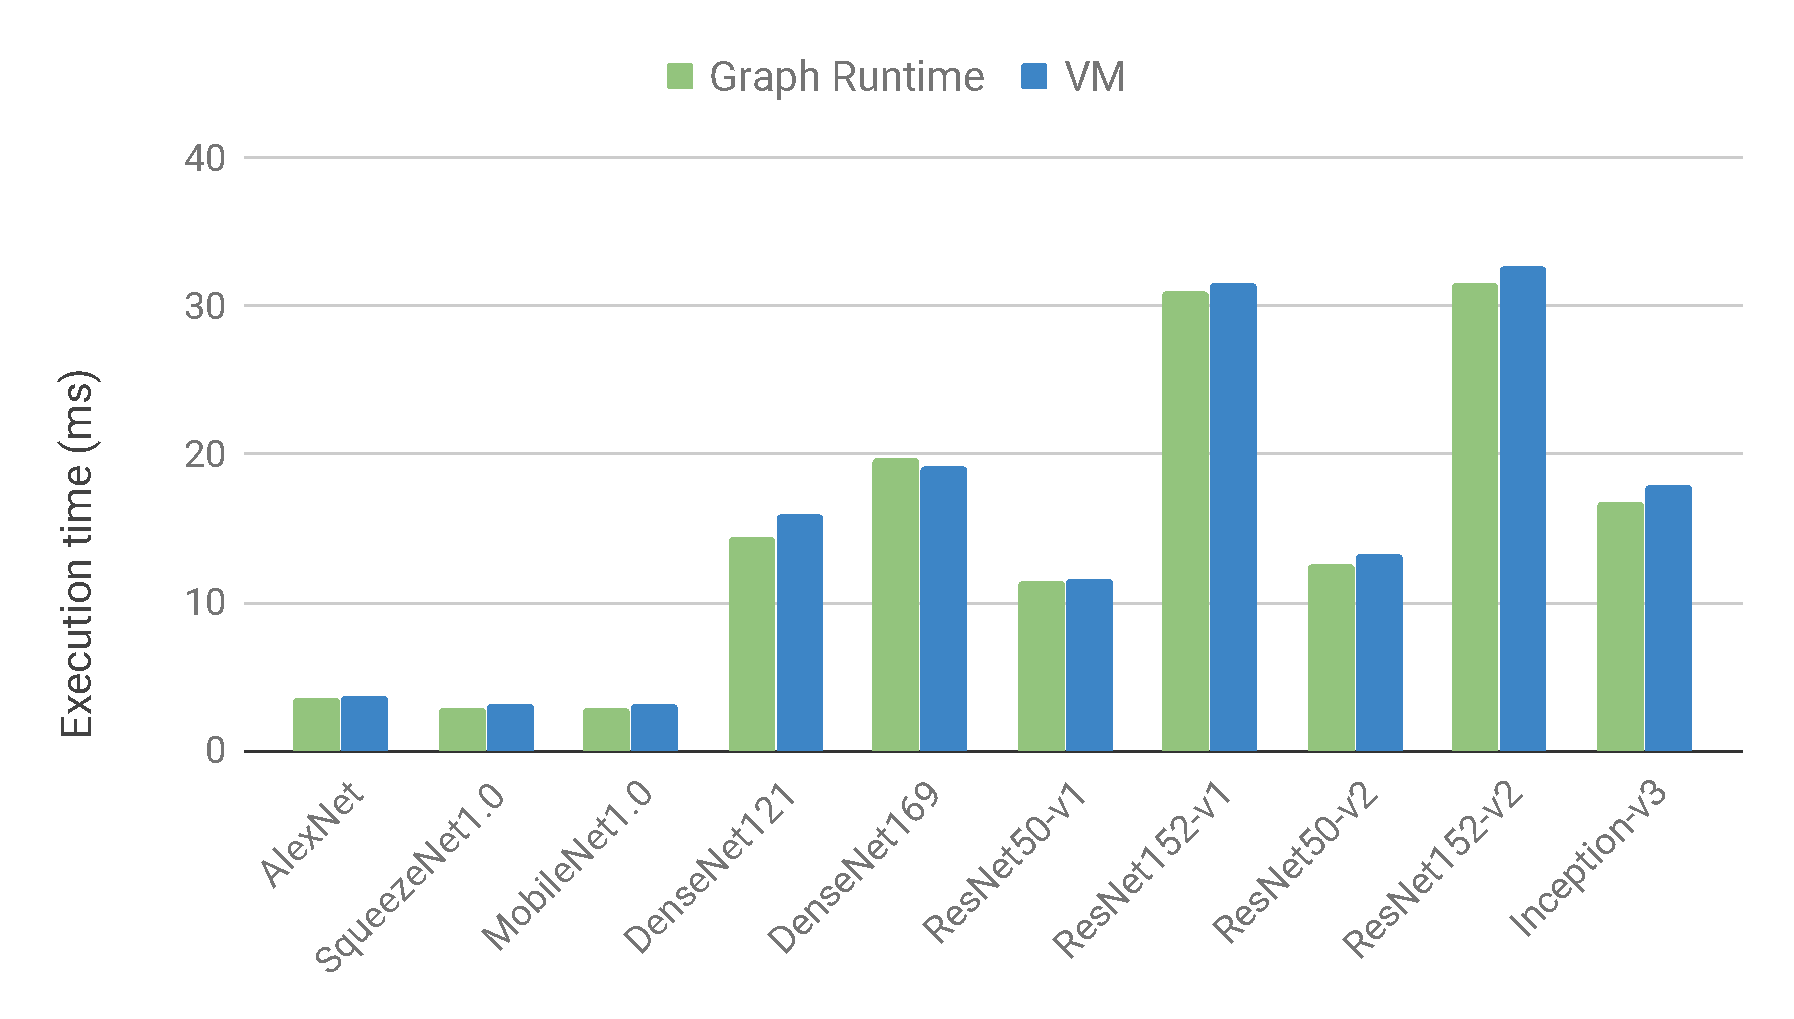
\includegraphics[width=.8\linewidth]{figs/cv_models.pdf}
      \caption{Benchmarking results of graph runtime vs. Relay.}
      \label{fig:benchmark}
    \end{figure*}

    \begin{table*}[t]
    \centering
    \begin{tabular}{llllrrc}
    \toprule
    \multicolumn{1}{c}{\multirow{2}{*}{input size}} & \multicolumn{1}{c}{\multirow{2}{*}{hidden size}} & \multicolumn{1}{c}{\multirow{2}{*}{\# layers}} & \multicolumn{1}{c}{\multirow{2}{*}{seq length}} & \multicolumn{2}{c}{latency (ms)}                         & \multicolumn{1}{c}{\multirow{2}{*}{speedup ($\times$)}} \\
    \multicolumn{1}{c}{}                            & \multicolumn{1}{c}{}                             & \multicolumn{1}{c}{}                          & \multicolumn{1}{c}{}                            & \multicolumn{1}{c}{MxNet} & \multicolumn{1}{c}{Relay VM} & \multicolumn{1}{c}{}                             \\
    \midrule
    100                                             & 100                                              & 1                                             & 1                                               & 0.53                      & 0.03                         & 18.4                                             \\
    100                                             & 100                                              & 1                                             & 20                                              & 4.74                      & 0.52                         & 9.2                                              \\
    100                                             & 100                                              & 1                                             & 100                                             & 21.75                     & 2.57                        & 8.5                                              \\
    100                                             & 100                                              & 2                                             & 100                                             & 30.53                     & 4.79                         & 6.4                                              \\
    100                                             & 100                                              & 3                                             & 100                                             & 55.47                     & 7.04                         & 7.9                                              \\
    200                                             & 600                                              & 3                                             & 100                                             & 67.14                     & 35.16                        & 1.9                                              \\
    400                                             & 1150                                             & 3                                             & 100                                             & 166.54                    & 123.54                       & 1.3                                              \\
    1500                                            & 1500                                             & 2                                             & 100                                             & 182.71                    & 138.78                       & 1.3
    \\\bottomrule
    \end{tabular}

    \caption{Compare performance of LSTM models between MxNet and Relay VM.}
    \label{tab:lstm}
    \end{table*}

    We evaluated the model inference with the VM against the TVM graph runtime on a number of popular vision models, including AlexNet, ResNet, MobileNet, VGG, DenseNet, SqueezeNet and Inception. Models are from GluonCV model zoo.  We repeated the inference 100 times for each model, obtained the performance result by averaging the execution times. All experiments were performed on Amazon EC2 C5.9xlarge instance (Intel Skylake-SP, 72 GiB memory, 18 physical cores, featured with AVX-512). In general, VM reached comparable inference performance even some optimizations were not plugged. As shown in \autoref{fig:benchmark}, we observed VM provided 2.59\% performance improvement on DenseNet169. On the rest of models, VM introduced some performance regression. We saw 11.3\% performance drop on SqueezeNet1.0.

    We also evaluated the inference performance of recurrent models, which requires control flow support. We choose LSTM model \citep{hochreiter1997long} and vary the input size, hidden size, number of layers, and sequence length. We measured the execution time of LSTM models for both MxNet MKL 1.4.1 and Relay VM on Amazon EC2 C5.9xlarge instance. \autoref{tab:lstm} shows that Relay VM can achieve 6.4-18.4$\times$ speedup on small LSTM models and 1.3-1.9$\times$ speedup on larger models.
    \end{comment}

    \section{Evaluation}
    \label{sec:eval}

    This section evaluates the performance of Relay on dynamic models against existing state-of-the-art solutions, as well as discussing the role of the optimizations performed by Relay. Specifically, the section seeks to answer the following questions:
    \begin{enumerate}
        \item What is the overall performance of Relay for dynamic models when compared against state-of-the-art alternatives on various hardware platforms?
        %\item How much overhead does Relay introduce for static models on top of the state-of-the-art solutions?
        \item How much overhead does Relay VM introduce for handling dynamism at runtime?
        \item How effective are the proposed optimization techniques, such as memory planning and symbolic codegen?
    \end{enumerate}

    %\yida{Evaluate the execution time of the bytecode as a portion of the total execution time, to show that VM overhead is negligible}
    %\note{End-to-end: BERT, LSTM, Tree-LSTM on Intel CPU, ARM CPU, NVidia GPU; Relay-runtime vs. graph runtime. Optimization implication: Kernel dispatch or not; memory planning or not; number of dispatched kernels.}
    \subsection{Experiment setup}
    \label{sec:eval:setup}

    All experiments were conducted on Amazon EC2 instances. We evaluated Relay on three hardware platforms: Intel Skylake CPUs (c5.9xlarge, 18 physical cores, hereinafter called {\em Intel CPU}), Nvidia Tesla T4 GPUs (g4dn.4xlarge, 1 card, 2,560 CUDA cores, hereinafter called {\em Nvidia GPU}), and ARM Cortex A72 (a1.4xlarge, 16 physical cores, hereinafter called {\em ARM CPU}). Although all tests are done on the cloud, our results of ARM CPU are portable to the edge devices, e.g. Raspberry Pi, due to the same architecture. %All cores have uniform memory access.

    To study the efficiency of Relay in handling dynamic models, we compared it with mainstream deep learning frameworks, including TensorFlow (v1.15), MXNet (v1.6), PyTorch (v1.5) \footnotemark, as well as dynamic-specific systems TensorFlow Fold based on TensorFlow v1.0.
    \footnotetext{We use PyTorch v1.4 on ARM CPU because PyTorch v1.5 fails to build on ARM instance.}
    %For TensorFlow Fold, its execution latency would include the compilation time (\zhicomment{@haichen, we probably need a bit argument here for why compile time is included.}).
    We were unable to compare Relay with Cavs~\citep{xu2018cavs}, JANUS~\citep{jeong2019janus}, or Jeong et al.\citep{jeong2018improving} as none of them is open-source. No public deep learning compiler has claimed support for dynamic models.
    %For static models, TVM~\citep{tvm_osdi18} was selected as the baseline to investigate the cost of Relay since it represents the state-of-the-art performance for static models on CPUs~\citep{liu2019optimizing}.

    Three popular models that represent different classes of dynamism were chosen in this experiment, viz. LSTM~\citep{lstm} (dynamic control flow), Tree-LSTM~\citep{tree_lstm} (dynamic data structure), and BERT~\citep{devlin2018bert} (dynamic data shape).
    The input size / hidden size used in the LSTM and Tree-LSTM model are 300/512 and 300/150, respectively.
    %while we use input size 300 and hidden size 150 in the Tree-LSTM model.
    We used BERT base implementation.
    For LSTM and BERT, we used Microsoft Research's Paraphrase Corpus (MRPC)~\citep{dolan2005microsoft} with variable input lengths as our input dataset. For Tree-LSTM, we used the Stanford Sentiment Treebank (SST)~\citep{socher2013recursive} with various tree structures as the input dataset.
    %\note{missing model size, e.g. LSTM number of layers, length, BERT size}
    %For the measurement of the overhead on static models, we completed model inference for ResNet~\citep{he2016deep}, MobileNet~\citep{howard2017mobilenets}, VGG~\citep{simonyan2014very}, and SqueezeNet~\citep{iandola2016squeezenet} on the ImageNet dataset~\citep{deng2009imagenet}. Only one input is needed to feed to the system each time for the task of model inference.

    \subsection{Overall performance}
    \label{sec:eval:overall}
    We compare the overall performance of Relay against baselines for each dynamic models. Relay successfully accomplished inference for all models on all platforms. However, not all baseline systems could perform inference for these models. For instance, TensorFlow Fold was not designed to process LSTM and BERT hence no result was obtainable, and Tree-LSTM only runs on PyTorch and TensorFlow Fold as other frameworks cannot handle dynamic data structures. Finally the model inference of Tree-LSTM on Nvidia GPU was omitted as it's hard to saturate GPU compute capability due to too many control flows and its model size, making GPUs less favorable deployment targets.
    % typical use cases.

    The baseline systems all make use of third-party kernel libraries to achieve high-performance by leveraging the heavily hand-optimized operators. We observe that dynamic models are often well-optimized on a single platform but perform poorly in other frameworks or on other targets. However, Relay has the ability to select either the self-compiled kernels or the ones provided by third-party library based on which one maximizes performance. It uses dynamic dispatch logic to invoke the selected kernels using platform-independent bytecode at runtime. This enables Relay to deliver portable and consistent results as many compiler optimizations are platform agnostic.
    %, and Relay has the freedom to choose whatever implementation that produces better performance.

    First, the latency results of Relay, MXNet, PyTorch, and TensorFlow on LSTM are shown in \autoref{tab:lstm}. Relay consistently outperforms the baseline on both 1- and 2-layer cases. For example, it reduces the latency of 1-layer LSTM model inference by $\fpeval{round(79.3 / 47.8, 1)}\times$, $\fpeval{round(212.9 / 47.8, 1)}\times$, and $\fpeval{round(301.4 / 47.8, 1)}\times$ over PyTorch, MXNet, and TensorFlow on Intel CPU,
    and $\fpeval{round(110.3/93.0, 1)}\times$, $\fpeval{round(135.7/93.0, 1)}\times$, $\fpeval{round(304.7/93.0, 1)}\times$ on Nvidia GPU, respectively.
    %On Nvidia GPU, Relay reduces the latency by  over PyTorch, MXNet, and TensorFlow on Nvidia GPU, respectively.
    On ARM CPU, Relay decreases the latency numbers even more remarkably, i.e. $\fpeval{round(1729.5 / 182.2, 1)}\times$ over PyTorch, $\fpeval{round(3695.9 / 182.2, 1)}\times$ over MXNet, and $\fpeval{round(978.3 / 182.2, 1)}\times$ over TensorFlow, respectively.
    The similar trend applies to 2-layer case of the LSTM model.
    We observe that latency on Nvidia GPU is higher than Intel CPU. This is because the size of LSTM model is relative small so that it cannot fully utilize the massive parallelism in the GPU.
    The significant performance improvement is due to Relay encoding the control flow into platform-independent instructions that have minimal overhead while deep learning frameworks use control flow specific primitives to process the sequence, which introduces a large performance penalty.

    \begin{table}[t]
    \centering
    \small
    \begin{tabular}{p{0.9cm}|ccc|ccc}
    \toprule
    Unit: & \multicolumn{3}{c|}{1 layer} & \multicolumn{3}{c}{2 layers} \\
    $\mu$s/token & Intel & NV & ARM & Intel & NV & ARM \\ \midrule
    Relay & \bf{47.8} & \bf{93.0} & \bf{182.2} & \bf{97.2} & \bf{150.9} & \bf{686.4} \\
    PT & 79.3 & 110.3 & 1729.5 & 158.1 & 214.6 & 3378.1 \\
    MX  & 212.9 & 135.7 & 3695.9 & 401.7 & 223.8 & 7768.0 \\
    TF & 301.4 & 304.7 & 978.3 & 687.3 & 406.9 & 2192.8 \\
    \bottomrule
    \end{tabular}
    \caption{LSTM model inference latency of Relay, PyTorch (PT), MXNet (MX), and TensorFlow (TF) on Intel CPU, Nvidia (NV) GPU, and ARM CPU.}
    \label{tab:lstm}
    \end{table}

    Next, we inspect the performance of model inference on Tree-LSTM as exhibited in \autoref{tab:treelstm} by comparing Relay with PyTorch and TensorFlow Fold. The table shows that Relay runs substantially faster than the baselines. On PyTorch, the performance speedups are $\fpeval{round(701.1/40.3, 1)}\times$ on Intel CPU and $\fpeval{round(1711.1/86.3, 1)}\times$ on ARM CPU as PyTorch uses Python to handle the tree data structure. TensorFlow Fold is $\fpeval{round(209.9/40.3, 1)}\times$ slower than Relay on Intel CPU because it has to re-compile upon every input.

    \begin{table}[t]
    \centering
    \begin{tabular}{l|ll}
    \toprule
    Unit: $\mu$s/token        & Intel     & ARM \\ \midrule
    Relay  & \bf{40.3}  & \bf{86.3}  \\
    PyTorch & 701.6 & 1717.1  \\
    TF Fold & 209.9 & --  \\
    \bottomrule
    \end{tabular}
    \caption{Tree-LSTM model inference latency on Intel CPU and ARM CPU. TensorFlow Fold was not built successfully on ARM CPU.}
    \label{tab:treelstm}
    \end{table}

    Third, \autoref{tab:bert} summarizes the performance of BERT for Relay, MXNet, and TensorFlow. The results indicate that Relay outstrips the baselines for all frameworks on all platforms in the experiment. The reduction in latency compared to the best framework on each platform is $\fpeval{round(455.8/307, 1)}\times$, $\fpeval{round(2995.4/2862.6, 2)}\times$, and $\fpeval{round(125.2/95.2, 1)}\times$ on Intel CPU, ARM CPU, and Nvidia GPU, respectively.
    %Surprisingly, Relay is $\fpeval{round(455.8/307, 1)}\times$ faster than MXNet on Intel CPU even the latter was known to be heavily optimized on this platform~\footnote{\url{https://medium.com/apache-mxnet/optimization-for-bert-inference-performance-on-cpu-3bb2413d376c}}.
    The reasons are two-fold: (a) similar to frameworks, Relay is also able to use the well-tuned third-party libraries on Intel CPU (MKL) and Nvidia GPU (cuDNN). (b) Relay can further enjoy the benefit of powerful operator fusion brought by the deep learning compiler. One can observe that we obtained more speedups on the ARM CPU for PyTorch and MXNet as the third-party libraries performed less favorable. However, Relay is only slightly faster than TensorFlow on the ARM CPU. This is because the dense operators (contributing to more than 90\% of the overall latency in Bert) on the ARM CPU was not well optimized by the underlying compiler. Therefore, the performance of the combination of operators it selected is on par with the ones used by TensorFlow.

    In sum, the evaluation results demonstrate that Relay produces more portable performance for all dynamic models on different platforms. Instead, the performance of frameworks is more platform dependent and varies from model to model.

    \begin{table}[t]
    \centering
    \begin{tabular}{l|lll}
    \toprule
    Unit: $\mu$s/token    & Intel  &   Nvidia       &  ARM     \\ \midrule
    Relay     & \bf{307.0} & \bf{95.2} & \bf{2862.6} \\
    PyTorch & 479.5 & 220.4 & 11851.2 \\
    MXNet      & 455.8 & 152.9 & 8628.0   \\
    TensorFlow & 768.7 & 125.2 & 2995.4 \\
    \bottomrule
    \end{tabular}
    \caption{BERT model inference latency on Intel CPU, Nvidia GPU, and ARM CPU.}
    \label{tab:bert}
    \end{table}

    % \begin{figure}[t]
    %     \centering
    %     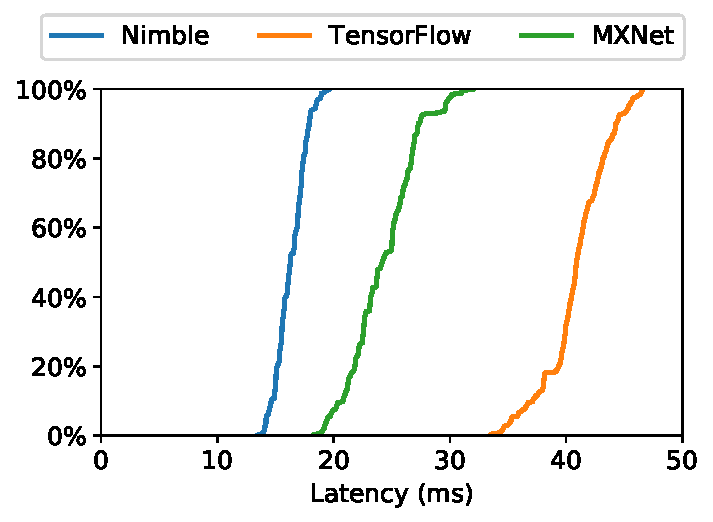
\includegraphics[height=5cm]{figs/bert_cdf_c5.pdf}
    %     \caption{BERT latency CDF on Intel CPU.}
    %     \label{fig:bert-cdf}
    % \end{figure}

    %\subsection{Optimization implications}
    %\label{sec:eval:opt}
    %\subsubsection{Memory planning}

    %\subsubsection{Dynamic kernel dispatch}
    \subsection{Microbenchmark}

    % \begin{table}[t]
    %     \centering
    %     \begin{tabular}{c|cc|cc}
    %         \toprule
    %         \multirow{2}{*}{Device} & TVM & Relay  & kernel & others  \\
    %         & lat. (ms) & lat. (ms) & lat. (ms) &  (ms) \\ %&  (\%) \\
    %         \midrule
    %         Intel  & 19.38 & 24.32 & 21.06 & 3.26 \\% & 13.4\%
    %         ARM & 223.50 & 237.41 & 228.59 & 8.82 \\%& 3.72\% \\
    %         Nvidia & 5.58 & 5.86 & 5.60 & 0.26 \\%& 4.44\% \\
    %         \bottomrule
    %     \end{tabular}
    %     \caption{BERT model latency (sequence length 128) using TVM and Relay on different hardware.
    %     {\it kernel latency} shows the latency of kernel invocation in Relay, and {\it others} shows the extra latency introduced by other instructions.
    %     }
    %     \label{tab:overhead}
    %
    % \end{table}

    % \hide{
    % \begin{figure}[t]
    %     \centering
    %     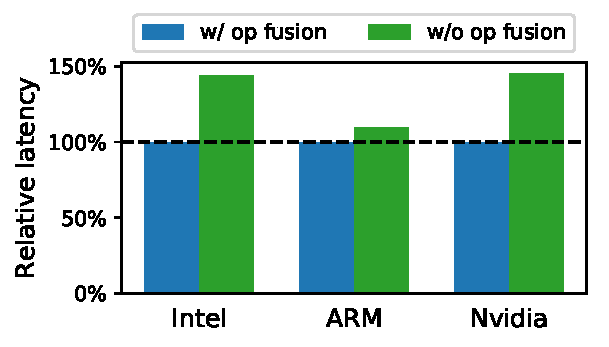
\includegraphics[height=3.5cm]{figs/op_fusion.pdf}
    %     \caption{Relative latency comparison between Relay with and without operator fusion for BERT model with sequence length 128.}
    %     \label{fig:fusion}
    %
    % \end{figure}
    % }

    \begin{figure}[t]
        \centering
        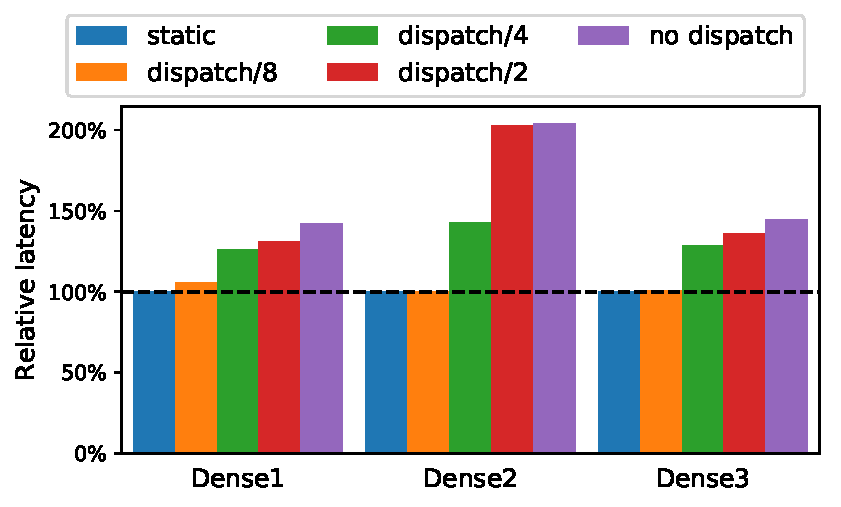
\includegraphics[height=4.5cm]{figs/sym_codegen.pdf}
        \caption{Relative latency comparison between symbolic codegen and static codegen of 3 dense operators on ARM CPU. The latency of kernel compiled with static shapes is used as the baseline. ``dispatch/$k$'' indicates that we generate $k$ symbolic kernels to be dispatched at runtime. ``no dispatch'' means that only one symbolic kernel is generated and therefore no dispatching is needed. %\protect\yida{The labels of x-axis, can we make them Dense 1, Dense 2 and Dense 3? L1, L2, L3 are like cache level to me at the first glance}
        }
        \label{fig:sym-codegen}
    \end{figure}

    This section analyzes the performance gain of Relay by using BERT as the microbenchmark. Three studies will be conducted to examine (a) the overhead introduced by the VM, %(b) the effectiveness of operator fusion\yida{Can we somehow relate this to any proposed techniques? For example, op fusion is enabled by carefully taking care of shape functions?},
    (b) the advantage of the proposed memory planning pass, and (c) the performance discrepancy between symbolic and static codegen.

    \noindent {\bf Overhead in handling dynamism} In order to understand the overhead that Relay spends to take care of dynamism, we compared it to TVM where static sequence length and TVM static runtime is used to execute BERT.


\section{Supporting Hardware Accelerators}
\label{sec:accel}

\subsection{Bring Your Own Code Generation}
\label{sec:byoc}

In conjunction with my collaborators at AWS we implemented an
  extensible framework for hooking hardware accelerators into
  TVM.
Bring Your Own Code Generation (BYOC) is a mechanism introduced
  into Relay for offloading specific sub-programs to hardware
  accelerators which operate outside of the traditional TVM
  programming model.

TODO

\subsection{VTA}
\label{sec:vta}

Hardware specialization is a powerful way to accelerate
  a known set of applications and workloads.
A component of Relay is lowering high-level programs down
  to the bespoke semantics of emerging hardware accelerators.
Unfortunately, deep learning (DL) is anything but a static field, and the machine learning (ML) community
  rapidly changes how they use to write models, the architecture of models themselves, the operators
  used by said models, and the data types they operate over.
Initial programmable accelerators~\citep{tpuv1} offer potentially huge performance
  improvements at the cost of complex specialized compilation.
Furthermore the churn of machine learning has lead to an interest
  in customizable designs, with features such as new numeric representations,
  new hardware engines, and more.
In order to customize the behavior of accelerators designs, even when open-sourced,
  there is a need for the availability of a transparent and modular software stack.
An end-to-end approach requires integration of frameworks, systems, compilers,
  and architecture in order to execute state-of-the-art ML using hardware acceleration.
Peak FLOPs provide value only if a programmer can access them.
In order to tackle this problem I have collaborated on the design for \vta (Versatile Tensor Accelerator),
  an explicitly programmed accelerator paired with a compiler and runtime that can evolve
  in tandem with deep learning models without sacrificing the advantages of specialization.

\vta makes following contributions:

\begin{itemize}
    \item \emph{A programmable accelerator design} that exposes a two-level programming interface: a high-level task ISA to allow explicit task scheduling by the compiler stack, and a low-level microcode ISA to provide software-defined operational flexibility.
    In addition, the \vta architecture is fully parameterizable: the hardware intrinsics, memories, and data types can be customized to adapt the hardware backend requirements.
    \item \emph{An extensible runtime system} for heterogeneous execution that performs JIT compilation of microcoded kernels to provide operational flexibility. For example, the \vta runtime lets us extend the functionality of \vta's original computer-vision-centric design to support operators found in style transfer applications without requiring any hardware modifications.
    \item \emph{A schedule auto-tuning platform} that optimizes data access and reuse in order to rapidly adapt to changes to the underlying hardware and to workload diversity.
\end{itemize}

My collaborators and I published a paper on VTA in
  the IEEE Micro Journal Special Issue on Deep Learning Acceleration~\citep{moreau2018vta}.
\vta and its children projects are a critical part of the research
  agenda at UW SAMPL lab, and we won a multi-million dollar grant to
  pursue automatically mapping Relay programs to hardware designs.
This work is being continued at UW and its one exciting future
  direction we discuss in Chapter~\ref{ch:future}.
